% !TEX root=template.tex

%Arquitetura: 

%Fazer descrição do sistema como um todo, incluir os diagramas já feitos. (MAS e ME) DONE

%Criar diagramas a explicar como o sistema em determinados use cases (durante desenvolvimento, manutenção, integração de novos agentes, etc) (ME) DONE

%TODO: Diagrama de componentes com os vários componentes do sistema e quem é que tem interfaces com quem (ME)

%TODO: Diagrama de atividades onde demonstras a evolução do sistema ao longo do tempo, para que o leitor perceba como este evolui, decisões, etc. (MAS e ME) (Sequence Diagrams)

%TODO: Descrever que o sistema foi desenhado tendo em conta a arquitetura com estes três agentes (RA, PA, TA) e que o RA e TA são os únicos que instanciam module engines. (MAS e ME)

%TODO: Explicar que os agentes utilizam o conceito de skill para que os RAs e TAs disponibilizem as suas capacidades e para que os PAs encontrem e peçam as capacidades que precisam. (MAS)

%TODO: Depois explicar como é que isto tudo funciona já com os agentes em causa. (MAS e ME) (Sequence Diagrams já feitos)



\typeout{NT FILE architecture.tex}

\glsresetall

\prependtographicspath{{Chapters/Figures/}}

\chapter{Architecture}
\label{cha:architecture}

In this section, the developed architecture is explained. Starting with an overview of the system, we will take a look at the main architecture, followed by a few use cases. Then we will go into more detail as to how each component of the system works and how they are connected through the interfaces it uses to communicate with other components. The evolution over time is also shown, to explain how the system might change and what kind of processes it undergoes. Finally, the supporting \acrlong{MAS} that was built to showcase the Module Engine is explained. Every agent is explained in detail and a full system architecture is presented at the end.

\section{System Architecture}
\label{sec:developed_architecture}

The system proposed in this work consists of two main components, a Module Engine and the Link Libraries. The Module Engine operates between the layers of software, in this case the agent, and hardware. It allows the agent to interface with any kind of hardware through the use of Link Libraries.\\

These libraries are what actually communicates to the hardware below, and can use any kind of communication protocols. Due to their modularity, any Link Library can be used at any point, independent of the characteristics of the agents above them. They are made with flexibility in mind to allow for the integration of any kind of hardware.\\

The Module Engine must be equally as flexible to allow for switching on the fly, during system operations. This allows for a more flexible and adaptable \acrshort{MAS}, since communications protocols can be switched fairly easy, the system becomes more robust also. In Figure~\ref{fig:system_architecture}, we can see the four main layers of the system. As we can observe, it matters not what kind of agent or hardware the agent is using, with the Module Engine, it must be capable of interfacing with it. 

\begin{figure}[h!]
	\centering
	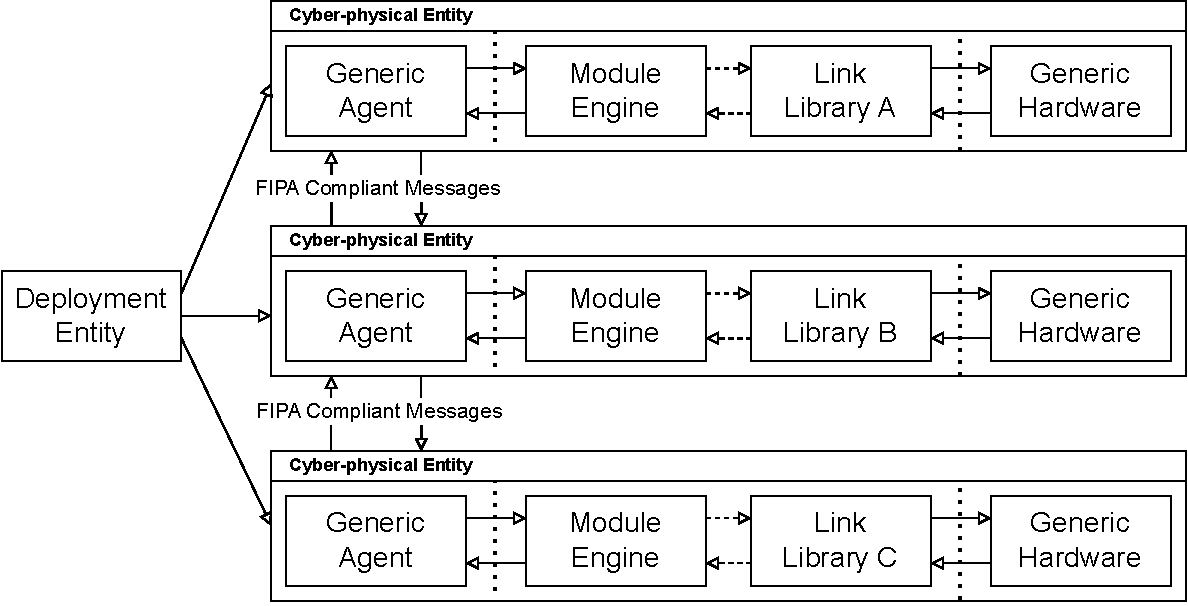
\includegraphics[scale=1]{System_Architecture}
	\caption{Simplified system architecture.}
	\label{fig:system_architecture}
\end{figure}

\section{Use Cases}
\label{sec:use_cases}

This system has three main use cases. The first is when a developer is creating a new agent to add to either a new system or a previously existing one. The second is when a developer wants to create a new Link Library to integrate a new type of hardware, or to use a different communications protocol. The third is when the already operating \acrshort{MAS} runs into an hardware problem, and needs to use other types of hardware to reduce system downtime. This use case can also be applied when a new agent is integrated into the already operating \acrshort{MAS}, since it is in part what is happening when an agent needs replacement.\\

When a developer is creating a new agent, they need to make sure to use the Module Engine together with the agents that need to interface to the hardware. For obvious reasons, those agents that do not use hardware do not need the Module Engine. They also need to make sure that the Link Library they wish to use to communicate is already developed. If not, then they need to create it. The creation of new Link Libraries will be explained below, in another use case. 

The agent will be able to call the Module Engine at any point during its operation, whenever it need to communicate something to the hardware. Figure~\ref{fig:me_dev_use_case} shows a diagram representing this use case. As we can see, the development of the agent is unrelated to the hardware. This is one of the advantages of the Module Engine. They can both be done in parallel to speed up development time.\\

\begin{figure}[h!]
	\centering
	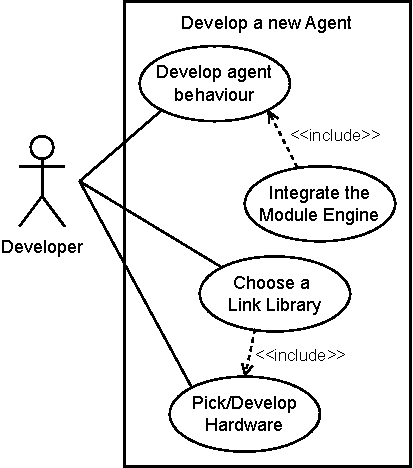
\includegraphics[scale=1]{ME_Dev_Use_Case}
	\caption{New agent development use case.}
	\label{fig:me_dev_use_case}
\end{figure}

Developing a new Link Library is fairly easy in comparison. The developer only needs to pick a new protocol and start development. Testing must be part of it, to make sure the new Link Library can in fact communicate with the Module Engine. When development is complete, this new Link Library can be published in some software distribution system, GitHub for instance, to be freely available to other developers wishing to use it. This use case can be seen in Figure~\ref{fig:ll_dev_use_case}.\\

\begin{figure}[h!]
	\centering
	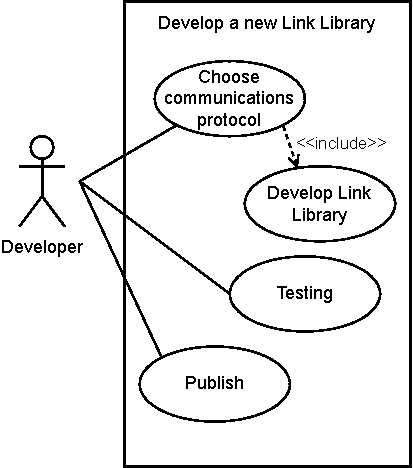
\includegraphics[scale=1]{LL_Dev_Use_Case}
	\caption{New agent development use case.}
	\label{fig:ll_dev_use_case}
\end{figure}

Finally, performing maintenance on a system using the Module Engine reduces system downtime, since if and when there is a fault, new hardware can easily be integrated. The Module Engine allows this, since Link Libraries more flexible than other hardware integrations, they can be replaced easily by selecting a different library from the already available ones. If there is not an adequate Link Library, a new one can be developed. Since they are relatively small, it might be faster to create a new library than to create a new interface for the hardware. It also follows that integrating new agents into the pre-existing \acrshort{MAS} is as easy, since both processes share similarities, as shown in Figure~\ref{fig:agent_maintenance_use_case}.\\

\begin{figure}[h!]
	\centering
		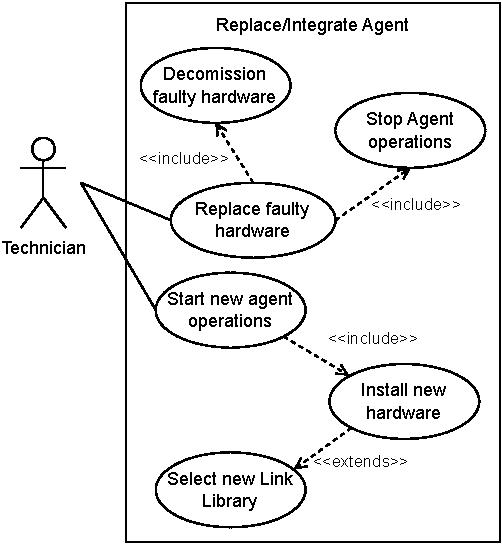
\includegraphics[scale=1]{Agent_Maintenance_Use_Case}
	\caption{Agent replacement/integration use case.}
	\label{fig:agent_maintenance_use_case}
\end{figure}

\section{System Components}
\label{sec:system_components}

The developed system is to be inserted between agent and hardware layers to allow for a more flexible interface. The cyber-physical entity of which the agent is part of is composed of four main components. The agent itself, the Module Engine tasked with loading the Link Libraries, the Link Libraries capable of interfacing with the hardware, and the hardware represented by the agent. The agent, the Module Engine and the Link Library can be considered the cyber part of the cyber-physical entity, with the hardware being the physical part.\\

In Figure~\ref{fig:component_diagram}, we can also see a Deployment Entity. This component is part of the overall \acrshort{MAS} and is detached from the agent. It is used to launch the agent and also provide it with the initial parameters. These parameters allow the Module Engine to select which Link Library is to be used and also give the Link Library its configurations needed to establish a connection to the hardware.\\

\begin{figure}[h!]
	\centering
	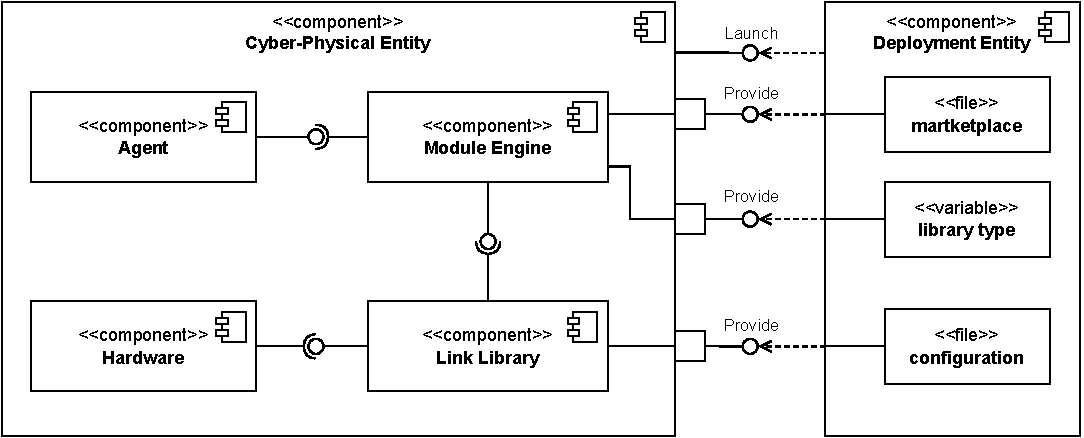
\includegraphics[scale=0.80]{Component_Diagram}
	\caption{Component diagram of a cyber-physical entity using the Module Engine.}
	\label{fig:component_diagram}
\end{figure}

\section{Module Engine Operations}
\label{sec:module_engine_operations}

The Module Engine is instantiated by the agent it is under. As explained before, the Module Engine needs three main components to operate. It needs the marketplace file, where all available Link Libraries are listed. From this list, the Module Engine picks the one to use based on the library type it also receives. Finally, after loading in the correct Link Library, it provides it with the configurations file.\\

The Link Library will now read this file and search for the configurations of the protocol it is implementing. It is possible to include more than one type of protocol in each configuration file. That is, a single configuration file may include different configurations for different protocols, but never more than one group of configurations per protocol. This file may include things like server addresses, ports, namespaces, topics, etc. Anything that the Link Library needs to establish a connection through the protocol it is implementing must be included in the configurations file.\\

Once communication with the hardware is established, the Module Engine will wait until a new command arrives from the agent. Once it does, it will pass that command downward to the Link Library, which will pass it along to the hardware. This process is needed to ensure modularity. Any Link Library can be associated with any agent, so the way to achieve this is to have an interface in the middle, the Module Engine, to pass instructions along.\\

Once the command is executed by the hardware, the result is passed along through the inverse path. From the hardware, to the Link Library, to the Module Engine and finally to the agent. This whole sequence of events is depicted in Figure~\ref{fig:module_engine_sequence_diagram}.

\begin{figure}[h!]
	\centering
	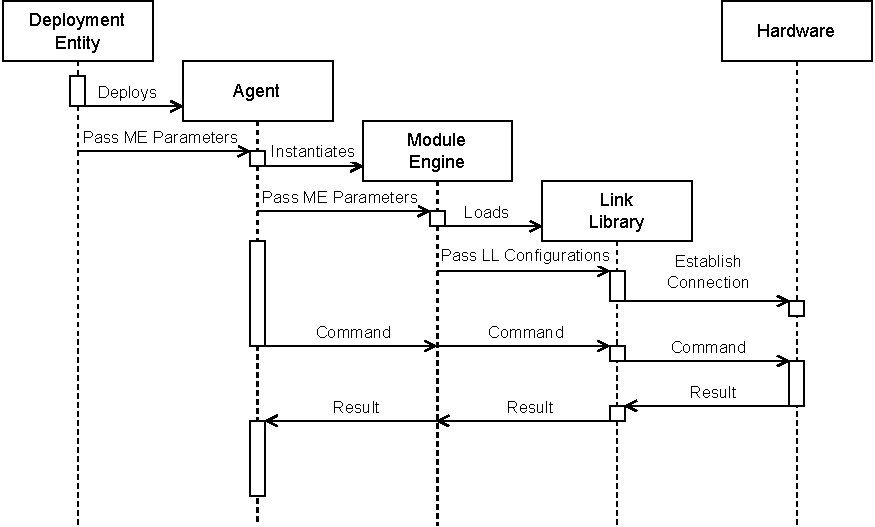
\includegraphics{Module_Engine_Sequence_Diagram}
	\caption{Sequence diagram of Module Engine operations.}
	\label{fig:module_engine_sequence_diagram}
\end{figure}

\section{Multi-Agent System}
\label{sec:multi-agent_system}

To showcase the functionalities and perform tests on the Module Engine, it was necessary to develop an Industrial \acrfull{MAS}. This \acrlong{CPPS} is composed of three main types of cyber-physical entities, with two other entities performing more of a management role, used for agent deployment. The two management entities are not considered cyber-physical entities because they do not have a physical counterpart and therefore do not use the Module Engine.\\

The developed entities are:
\begin{itemize}
	\item The \acrfull{RA}, that represents any kind of physical component capable of performing processes, like a robotic arm or a bottle filling station;
	\item The \acrfull{TA}, that represent any kind of physical component capable of transporting products from one location on the shop floor to another, components like a conveyor belt or a \acrfull{AGV};
	\item The \acrfull{PA}, that represent any kind of product to be manufactured by the Industrial \acrshort{MAS};
	\item The \acrfull{DA}, that will launch \acrshortpl{RA} and \acrshortpl{TA} and provide them with the necessary parameters. This is the entity seen in Figure~\ref{fig:component_diagram};
	\item And the \acrfull{PM}, that will launch \acrshortpl{PA} and provide them with their production sequence.
\end{itemize}


When the system is first launched, the agents that start up immediately are the \acrfull{DA} and \acrfull{PM}, since both of these agents are responsible for the launch and management of all other agents. Both of them need to be capable of receiving input from a human user through a \acrfull{GUI}. The user creates the necessary agents through the \acrshort{DA} by providing it with the Link Library type and configuration file. The \acrshort{DA} is capable of launching both \acrshortpl{RA} and \acrshortpl{TA} because these are the agents that need the Module Engine to operate as mentioned above. Figure~\ref{fig:da_activity_diagrams} presents the process of deploying a new agent (\ref{fig:da_activity_diagram_deploy_agent}) and stopping a pre-existing agent (\ref{fig:da_activity_diagram_stop_agent}). The marketplace file is not provided by the user, but could instead be provided by some kind of web application. For this work however, it is provided locally and the \acrshort{DA} has access to its contents directly.\\

\begin{figure}[h!]
	\centering
	\subbottom[Deployment of new agent.\label{fig:da_activity_diagram_deploy_agent}]{%
		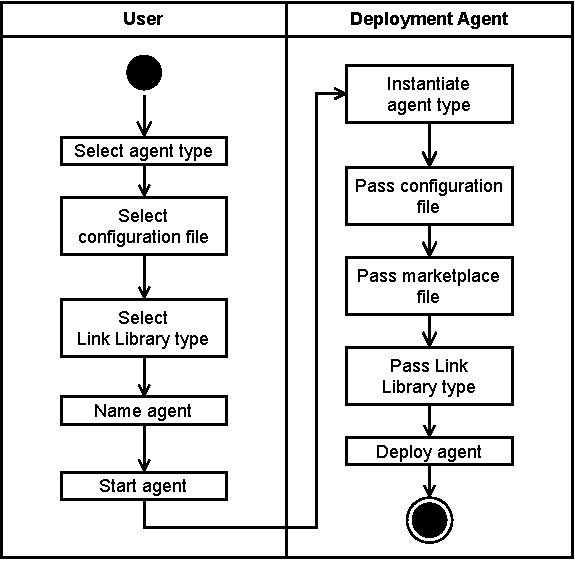
\includegraphics[width=0.5\linewidth]{Activity_Diagram_DA_deploy}}%
	\hspace{0.80cm}
	\subbottom[Stopping of running agent.\label{fig:da_activity_diagram_stop_agent}]{%
		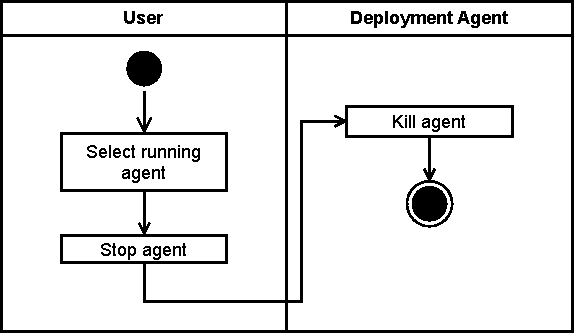
\includegraphics[width=0.5\linewidth]{Activity_Diagram_DA_stop}}%
	\caption{\acrlong{DA} activity diagram.}
	\label{fig:da_activity_diagrams}
\end{figure}

The \acrlong{PM} is simpler in its activities, since its only task is to launch \acrlongpl{PA}. A user only has to start the agent through the \acrshort{GUI} of the \acrshort{PM}. When a \acrshort{PA} is started, it does not need any other external parameters. Figure~\ref{fig:pm_activity_diagram} presents this simple operation. Since the \acrshort{PM} does not terminate the \acrshortpl{PA}, it only has the functionality to deploy agents.\\

\begin{figure}[h!]
	\centering
	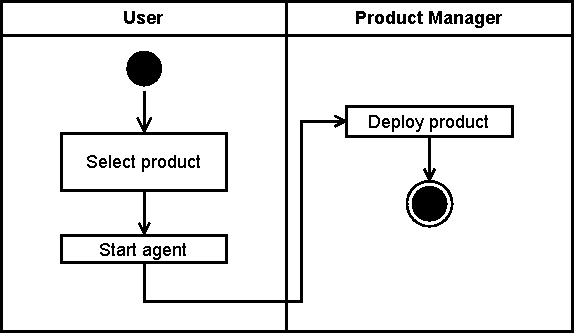
\includegraphics[scale=0.9]{Activity_Diagram_PM}
	\caption{\acrlong{PM} activity diagram.}
	\label{fig:pm_activity_diagram}
\end{figure}

After deployment, \acrlongpl{RA} and \acrlongpl{TA} will instantiate the Module Engine and pass it the marketplace and configuration files, along with the Link Library type. Then they will proceed to register themselves in the \acrlong{DF}, which is a way for agents to search for other agents with specific characteristics. This \acrshort{DF} works a little bit like a phone book, presenting all registered agents along with their agent ID, a unique identifier that corresponds to each agent. Any agent can access the \acrshort{DF} and search for agents with certain capabilities, called skills. These skills show what actions an agent can perform. For example, an agent with a skill called "Move\_to\_Storage" might move itself or a load to storage, or an agent with the skill "Staple\_tag" might be able to staple a tag on a piece of clothing, and so on. A production sequence is list of the skills a product needs to be performed in order to complete it fabricated. In the designed system, \acrlongpl{PA} can use the \acrshort{DF} to look for \acrshortpl{RA} and \acrshortpl{TA} capable of performing the needed skills.\\

When all \acrshortpl{RA} and \acrshortpl{TA} have been launched and their initial setup completed, the system is now ready to work. \acrshortpl{PA} are launched as new products enter the production line, and after getting their production sequences, they will search the \acrshort{DF} to find a \acrshort{RA} capable of performing the first skill. When they find it, they will issue a Call for Proposals from all relevant agents through the Contract Net. This interaction protocol was developed by \acrshort{FIPA}, and it works as follows:

In this protocol the agent that starts the communication is called the Initiator, and all other are the Participants. The Initiator sends a Call for Proposals or CFP message to all Participants preselected by the Initiator. After receiving the message, the Participants can either accept the call by sending a Proposal, or refuse altogether. On refusal, this particular Participant is out of communications from now on. Proposals might include some data to help the Initiator decide which Participants it wants to keep communicating with. Upon deciding this, the Initiator will send an Accept Proposal message to the desired Participants, Rejecting all other Proposals. Finally, the Participants whose Proposal was accepted might perform some process and inform the Initiator of the result, with a Failure message or a Inform message. This interaction protocol can be visualized in Figure~\ref{fig:contract_net_protocol}.\\

\begin{figure}[h!]
	\centering
	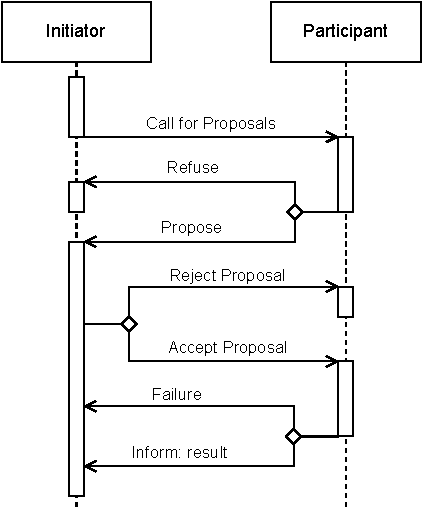
\includegraphics[scale=1]{FIPA_Contract_Net}
	\caption{Contract Net interaction protocol. Adapted from \cite{FIPA_Contract_Net}.}
	\label{fig:contract_net_protocol}
\end{figure}

After receiving the Call for Proposals, \acrshortpl{RA} will respond with a Proposal. This simply signifies that the agent is available to perform the needed skill, and it does not contain any extra data. Then the \acrshort{PA}, the Initiator, will Accept the first Proposal on the responses list for simplicity. Finally the selected \acrshort{RA} will respond with an Inform message, in which the contents of the message contain the location of the \acrshort{RA} on the shop floor. This location will be used by the \acrshort{PA} to ask for transportation from a \acrshort{TA}. An example of a communication through the Contract Net can be seen in Figure~\ref{fig:pa_ra_contract_net}. In this example, two \acrshortpl{RA} have the relevant skill for the \acrshort{PA}. It selects the first one and rejects the other. Then the \acrshort{RA} Informs the \acrshort{PA} of their location.\\

\begin{figure}[h!]
	\centering
	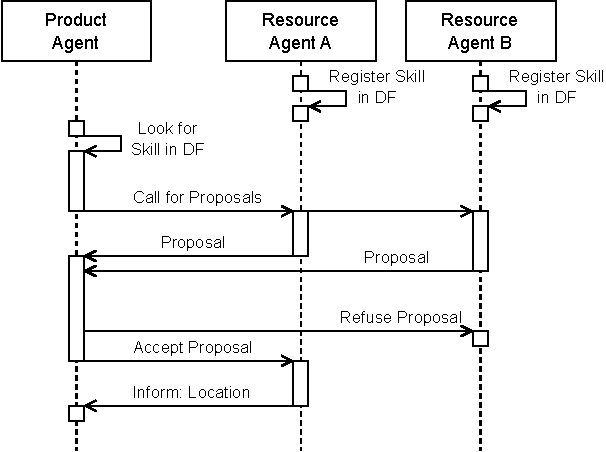
\includegraphics{PA_RA_Contract_Net}
	\caption{Contract Net protocol between a \acrlong{PA} and two \acrlongpl{RA}.}
	\label{fig:pa_ra_contract_net}
\end{figure}

Upon finding a \acrlong{RA}, the \acrlong{PA} now needs to be transported to its work station. For this it needs a \acrlong{TA}. So the \acrshort{PA} will once again look into the \acrshort{DF} for a \acrshort{TA}, by searching for a skill once again. It was decided that for simplicity, only one transport agent will be used in the simulated system. So instead of asking for an agent through the Contract Net, we can skip straight away to the next step, which is to ask for a skill to be performed through a Request. This protocol is also one created by \acrshort{FIPA}, and its less complex than the Contract Net:

This protocol also includes an Initiator, but only one Participant. This is a one to one communication. The Initiator starts by sending a Request to the Participant. At this point the Participant may Refuse, and communications are terminated. If it Agrees however, it will start performing the desired process immediately. Upon completion, it will notify the Initiator with either a Failure or Inform message. This protocol is shown in Figure~\ref{fig:requests_protocol}.\\

\begin{figure}[h!]
	\centering
	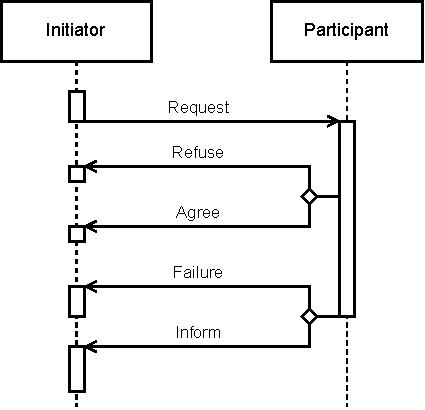
\includegraphics{FIPA_Requests}
	\caption{Request interaction protocol. Adapted from \cite{FIPA_Request}.}
	\label{fig:requests_protocol}
\end{figure}

The \acrshort{PA} sends a Request with its starting and ending positions, so the \acrshort{TA} from where the \acrshort{PA} departs from, and what is its destination. After Agreeing with the Request and before the communication terminates, the \acrshort{TA} will transport the \acrshort{PA} to the destination and send an Inform message signalling the transportation is complete. After arriving at the location where the previously found \acrshort{RA} is located, the \acrshort{PA} will  use the same protocol to Request the skill from the \acrshort{RA}. Both of these sequences of messages are shown in Figure~\ref{fig:agent_requests}. In \ref{fig:pa_ra_requests} we can see the Requests protocol between a \acrshort{PA} and \acrshort{TA}, and in \ref{fig:pa_ta_requests} between a \acrshort{PA} and \acrshort{RA}.\\

\begin{figure}[h!]
	\centering
	\subbottom[\acrlong{PA} and \acrlong{TA}.\label{fig:pa_ra_requests}]{%
		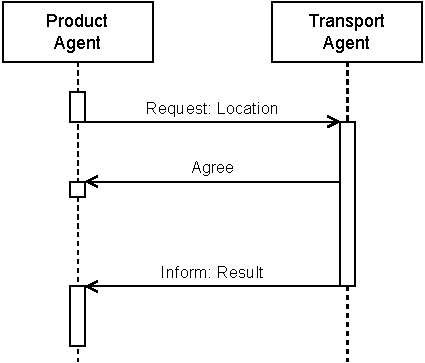
\includegraphics[width=0.5\linewidth]{PA_TA_Requests}}%
	\hspace{0.75cm}
	\subbottom[\acrlong{PA} and \acrlong{RA}.\label{fig:pa_ta_requests}]{%
		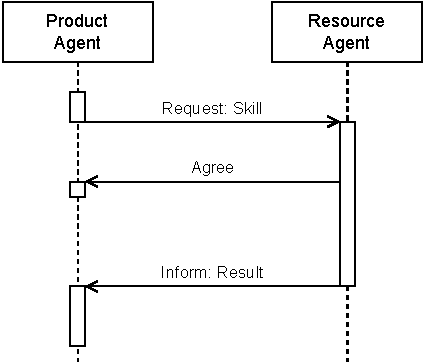
\includegraphics[width=0.5\linewidth]{PA_RA_Requests}}%
	\caption{Requests between agents.}
	\label{fig:agent_requests}
\end{figure}

When the \acrshort{RA} finishes it skill and informs the \acrshort{PA}, the \acrshort{PA} will check if its production sequence is complete. If it is, it will Request transportation from a \acrshort{TA} to storage. If the sequence is not complete, it restarts the process by checking the \acrshort{DF} for agents capable of performing the next skill, Calling for Proposals, and so on. The whole evolution of the \acrshort{MAS} can be visualized in Figure~\ref{fig:mas_activity_diagram}. It only shows the full interactions between agents, their actions and decisions without the Module Engine.\\

\begin{figure}[H]
	\centering
	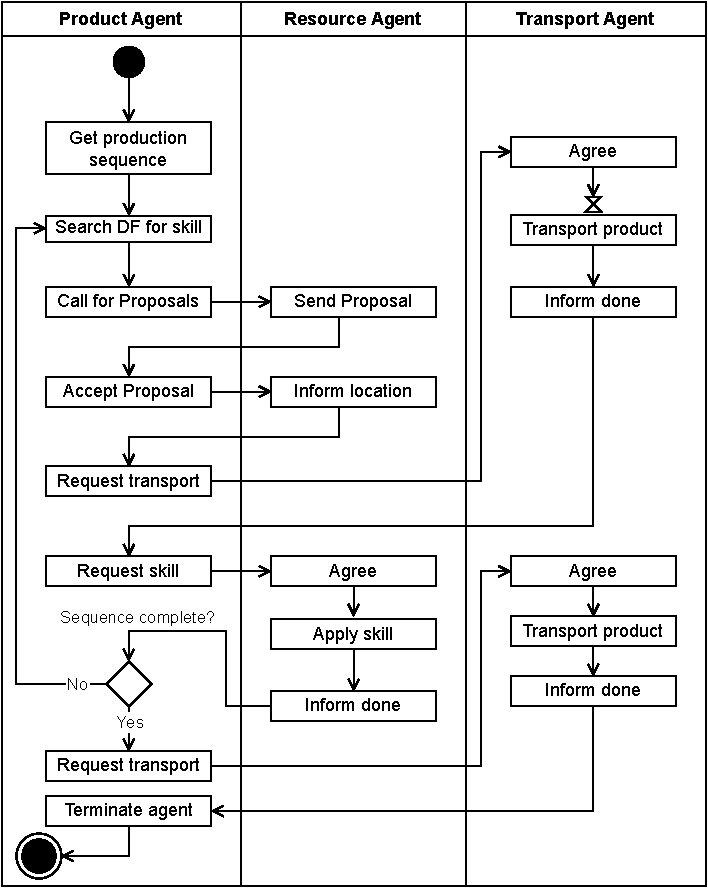
\includegraphics{MAS_Activity_Diagram}
	\caption{Activity diagram of the Industrial \acrlong{MAS}.}
	\label{fig:mas_activity_diagram}
\end{figure}

\section{System Overview}
\label{sec:system_overview}

Now that all parts of the system have been explained, we will do a brief overview of the behaviour of the system has a whole. When the \acrshort{MAS} is launched, the first two agents that start up immediately are the \acrlong{DA} and the \acrlong{PM}. Then a user needs to launch the \acrlongpl{RA} and the \acrlong{TA} and select the right configurations for each agent.\\ 

When these agents are launched, they will register themselves in the \acrshort{DF} with their skills and instantiate their Module Engine, which will in turn load the corresponding Link Library. These libraries will establish connection to the hardware. After all of these agents are deployed and ready to operate, the user can now launch the \acrlong{PA}.\\

Upon being launched, the \acrshort{PA} will look in the \acrshort{DF} and it will find the \acrshortpl{RA} capable of performing the first skill in its production sequence. Then it will establish contact with all of them through the Contract Net. After receiving the Proposals, it will select one and refuse the all others. In the last message, the \acrshort{PA} will receive the location of the station where the \acrshort{RA} is located.\\

The next step is to Request transportation from a \acrshort{TA} to this location. The \acrshort{PA} will issue a Request with its current location and its destination. The \acrshort{TA} will answer this Request to signal it received the message and will immediately start the process of moving the product. For this, it will send the command through the Module Engine and through the Link Library, to the hardware. Once the hardware finishes executing it, it will send the result back up through the Link Library and through the Module Engine to the agent.\\

The \acrshort{TA} will now notify the \acrshort{PA} that transportation is complete. The \acrshort{PA} then issues another Request, this time to the previously chosen \acrshort{RA}. This agent will execute its skill by using the same process as the \acrshort{TA}. Through the Module Engine and Link Library down to the hardware. After the result arrives back at the agent, it will notify the \acrshort{PA}. If this is the last skill in this products production sequence, the \acrshort{PA} will now Request another transportation, but this time to storage, terminating the agent and ending its production. If, however, there are still skills in the production sequence, then the process restarts. The \acrshort{PA} will search again for a \acrshort{PA} capable of performing the new skill in the sequence and so on. In Figure~\ref{fig:complete_activity_diagram}, this whole process is shown, from start to finish.\\

\begin{figure}[h!]
	\centering
	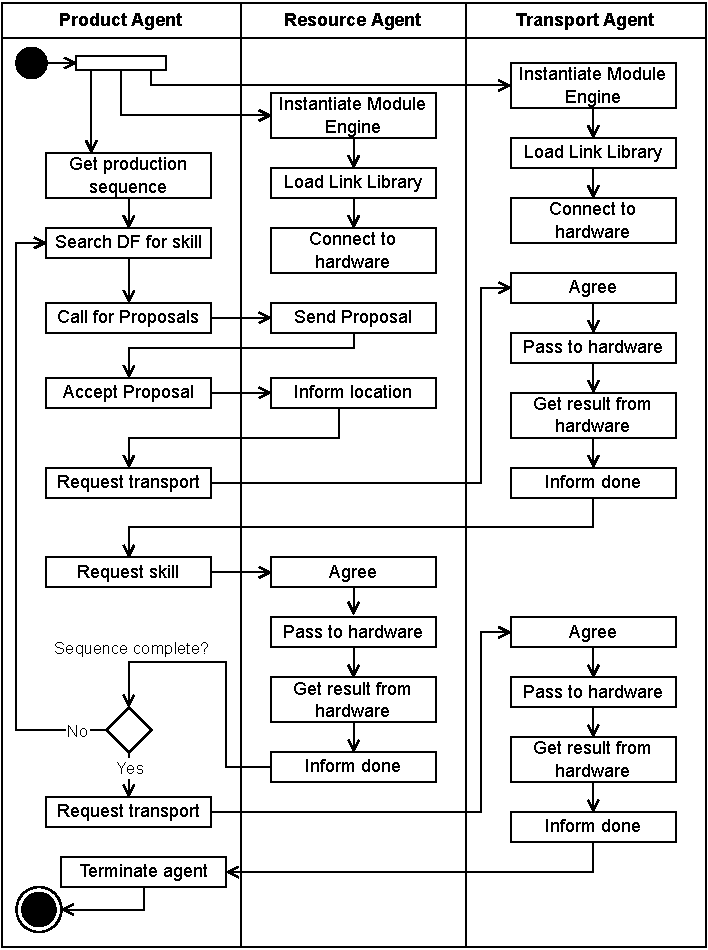
\includegraphics{Complete_System_Activity_Diagram}
	\caption{Activity diagram of the final system.}
	\label{fig:complete_activity_diagram}
\end{figure}
